\documentclass[a4paper,11pt]{article}
\usepackage{graphicx}
\usepackage{booktabs}
\usepackage{tabularx}
\usepackage{url}
\usepackage{pdfpages}
\usepackage{epstopdf}

\graphicspath{ {images_eps/} }

%
% Do not change
\textheight = 220mm
\textwidth  = 150mm
\topmargin  = 10mm
\oddsidemargin  = 5.0mm
\evensidemargin = 5.0mm
\unitlength = 1mm

\usepackage[utf8]{inputenc}
\usepackage[T1]{fontenc}
\usepackage[swedish]{babel}

\begin{document}
%
% Do not change
\let\rempage=\thepage
{
\renewcommand{\thepage}{\relax}
\begin{picture}(44,0)(15,10)
% \special{psfile=mahlogo-name.eps}
\includegraphics[scale=1]{mahlogo-name.eps}
\end{picture}

\vspace*{-30mm}
\hfill\begin{minipage}[t]{16em}\large
Fakulteten för teknik och samhälle\\
Datavetenskap
\end{minipage}

\vspace*{45mm}
\begin{center}
{\bf\large
Examensarbete 

\small
15 högskolepoäng, grundnivå
}

\vspace*{25mm}
\LARGE
%
% Put your title here
LEAP: Automatiserad bedömning av programmeringsuppgifter

\vspace*{8mm}
\large
%
% Translated title 
LEAP: Automatic assessment of programming assignments

\vspace*{12mm}
\Large
%
% Author names
Felix Alhbin\\
Mattias Pernhult

\vspace*{30mm}
\large
%
% Picture if you want
\end{center}

\vfill
\hspace*{-10mm}%
\begin{minipage}[t]{20em}
%
% Fill in correct data for you
Examen: Kandidatexamen 180~hp
\\
Huvudområde: Datavetenskap
%
% Huvudområden är:
% Affärssystem
% Data och informationsvetenskap (IA och IS)
% Datavetenskap (Övriga)
\\
Program: Systemutvecklare
\\
Datum för slutseminarium: 2016-05-30
\end{minipage}
%
\hfill
%
\begin{minipage}[t]{15,5em}
%
% Fill in supervisor and second reader
Handledare: Ulrik Eklund
\\
Andrabedömare: Magnus Krampell
\end{minipage}

\newpage

\mbox{}

\newpage

\section*{Sammanfattning}

Text på svenska\ldots

\newpage

\mbox{}

\newpage

\section*{Abstract}

Text in English\ldots

\newpage

\mbox{}

\newpage
\tableofcontents
\newpage
\ifodd\value{page}\else\mbox{}\newpage\fi
\setcounter{page}{1}
\renewcommand{\thepage}{\rempage}

\section{Inledning}

\subsection{Bakgrund}

Ett sätt att lära sig att programmera är genom introduktionskurser på universitetet. I sådana kurser ges studenter olika uppgifter som kan hjälpa dem att bli familjära med moderna programmeringsspråk, lära sig viktiga verktyg och få insikter om hur systemutveckling bedrivs \cite{douce_11}. Utvärdering och bedömning av dessa programmeringsuppgifter utförs vanligtvis manuellt av lärare och labbhandledare. När kurser utförs på detta traditionella sätt och de innehåller ett högt antal studenter skapar det tunga och tidskrävande uppgifter för lärare och övningsassistenter vilket tär på universitetets resurser. Det innebär även att återkopplingen till studenterna fördröjs vilket har en negativ påverkan på deras utveckling jämfört med direkt återkoppling \cite{japanerna_1}. Eftersom potentiella lösningar till mindre programmeringsuppgifter är av likartad karaktär kan utvärdering och bedömning automatiseras genom automatiserade bedömningssystem. Därav kan lärares resurser användas på ett mer effektivt sätt och på så vis förbättra kvalitén i kursens andra moment samtidigt som det ger en objektiv bedömning och direkt återkoppling till studenterna \cite{douce_11} \cite{hollingsworth_2} \cite{higgins_3}. Automatiserade bedömningssystem för programmeringsuppgifter nämns redan första gången 1960 av Hollingsworth \cite{hollingsworth_2}. Studenterna använde sig av hålkort med program skrivna i assembly som de skickade in för bedömning. Sedan dess har automatiserade bedömningssystem vidareutvecklats.

\subsection{Syfte}

Studien ämnar att implementera ett bedömningssystem som är tänkt att användas för introduktionskurser i programmering som bedrivs på Malmö Högskola. Syftet är dels att undersöka om vårt bedömningssystem kan underlätta och ge stöd åt lärare i deras bedömningsprocess av programmeringsuppgifter och dels att undersöka om vårt bedömningssystem är ett bra hjälpmedel för att utveckla studenters programmeringskunskaper.

\subsection{Frågeställning}

Studien avser ge svar på följande frågor:

\begin{enumerate}
\item
Kan ett automatiserat bedömningssystem av den här typen minska tidsåtgången för lärares bedömningsprocess av programmeringsuppgifter?
\item
Är ett automatiserat bedömningssystem av den här typen bättre för studenters programmeringsutveckling än traditionell bedömning?
\end{enumerate}

\newpage
\subsection{Hypotes}

Angående frågeställning 1 tror vi att det initialt krävs en del av lärares resurser och att det därför till en början inte lönar sig att använda ett bedömningssystem i programmeringskurser eftersom ett sådant system kräver att lärare exempelvis skriver testfall för att bedöma studenters uppgifter och att existerande uppgifter behöver modifieras. Vi tror dock på sikt att ett bedömningssystem minskar lärarnas tidsåtgång för bedömningsprocessen av programmeringsuppgifter.

Angående frågeställning 2 tror vi att direkt återkoppling gör ett automatiserat bedömningssystem till ett bättre val gällande studenters programmeringsutveckling jämfört med traditionell bedömning.

\subsection{Relaterat arbete}

Daly och Horgan \cite{roboprof_4} presenterar i sin artikel hur de utvecklade det automatiserade lärningssystemet RoboProf\cite{roboprof_4}. I artikeln utförde de även en studie där de testade att använda RoboProf i en introduktionskurs för programmering. Resultaten från studien visar att de studenter som utförde kursen på ett traditionellt vis presterade betydligt sämre än de studenter som använde RoboProf. Vidare presenterar författarna även en lösning för plagieringsproblemet vilket bygger på en idé av Plauger \cite{plaguer_5}.

I artikeln \cite{edwards_15} presenterar Edwards och Pérez-Quiñones deras erfarenheter av att använda testdriven utveckling med Web-CAT \cite{edwards_15}. Web-CAT är unikt bland automatiserade bedömningssystem eftersom det bedömer hur bra studenterna testar deras egen kod istället för att studenternas kod testas gentemot fördefinierade testfall \cite{edwards_15}.

Higgins m. fl. \cite{higgins_3} påpekar i sin studie om det automatiserade bedömningssystemet CourseMarker \cite{higgins_coursemarker_12} att studenter ofta vill ha detaljerad information om vilken del av deras kod som inte godkändes. Författarna hävdar dock att alltför detaljerad information i återkopplingen kan ha negativ påverkan på studenters resultat. CourseMarker löser problemet genom att låta läraren själv ange hur detaljerad återkopplingen till studenten ska vara \cite{higgins_3} \cite{caiza_7} \cite{douce_11}.

En alternativ lösning presenteras av Reek som begränsar antalet försök en student har på sig att genomföra en uppgift. Detta för att tvinga studenten att tänka över deras lösning mer noggrant innan de lämnar in den \cite{reek_6}. Denna lösning presenteras även av Ihantola m. fl. \cite{ihantola}.

Caiza och Del Alamo tar även de upp problem kring återkoppling till studenter \cite{caiza_7}. De nämner \textit{trial and error} problemet vilket betyder att studenter prövar sig fram genom att göra mindre förändringar i deras program istället för att reflektera över vad problemet beror på. Författarna påstår att de inte upplevt \textit{trial and error} beteendet bland de medverkande studenterna.

Ihantola m. fl. \cite{ihantola} lyfter fram olika lösningar för att förhindra \textit{trial and error} beteendet.  En alternativ lösning som de presenterar är att begränsa mängden återkoppling till studenten. Dock kan detta frambringa förvirring hos studenten eftersom studenten inte förstår varför programmet bedömdes som inkorrekt [26]. Vidare nämner författarna en lösning där studenten får en tidsbestraffning vid ett misslyckande, de påpekar även att tidsbestraffningen kan öka exponentiellt.
De presenterar även en lösning där studenten får en slumpmässigt utvald uppgift vid varje nytt försök vilket förhindrar \textit{trial and error} beteendet. 

Hollingsworth påpekar att studenters program kan innehålla skadlig kod vilket kan förstöra bedömningssystemet, de utgör därmed ett hot mot systemet \cite{hollingsworth_2}. Detta problem adresseras av artiklarna \cite{spacek_13} \cite{cs50_8} \cite{ihantola} där författarna presenterar två alternativa lösningar som bygger på grundtanken att kompilera och exekvera studenternas program i en säker miljö för att skydda bedömningssystemet. I artikeln \cite{cs50_8} presenterar Malan bedömningssystemet CS-50 vilket utvecklades som en del av en internetbaserad kurs vid Harvard Universitetet. För att säkert kompilera och exekvera opålitlig kod använder CS-50 SELinux \cite{selinux} och PAM begränsningar \cite{pambegransningar}. Špaček m. fl. \cite{spacek_13} hävdar i sin studie att flertalet av dagens bedömningssystem saknar stöd för exekvering av opålitliga program i en säker miljö. Författarna har i sin lösning valt att använda den virtuella containerbaserade plattformen Docker \cite{docker} för att kompilera och exekvera studenternas program. APAC verifierar studenternas program genom att analysera och validera programmets utdata.

\subsection{Avgränsning}

De respondenter och testpersoner som deltar i studien för att besvara forskningsfrågan är lärare och studenter på Malmö Högskola inom institutionen Datavetenskap.


\newpage
\section{Metod}

Följande avsnitt beskriver den metodik som valts för utförandet av studien.

\subsection{Metodbeskrivning och metoddiskussion}

Eftersom studiens syfte är att konstruera, implementera och utvärdera en systemartefakt valdes en metodik som presenteras av Nunamaker m. fl. \cite{nunamaker} eftersom det är en erkänd och välbeprövad process för forskning inom informationssystem. Författarna definierar en iterativ femstegsprocess för hur sådan forskning bör bedrivas vilken innefattar att: \textit{(1) konstruera ett konceptuellt ramverk} \textit{(2) utveckla en systemarkitektur} \textit{(3) konstruera och analysera systemet} \textit{(4) implementera systemet} och \textit{(5) utvärdera systemet}. För att ytterligare säkerställa studiens kvalité följer den de sju riktlinjer för forskning inom informationssystem definierade av Hevner m.fl. \cite{hevner}. 

\subsubsection*{Konstruera ett konceptuellt ramverk}

Syftet med att konstruera ett konceptuellt ramverk är att definiera en relevant forskningsfråga och systemkrav. För att identifiera och definiera dessa genomför vi en litteraturstudie av liknande system och intervjuar lärare vid Malmö högskola. Vi väljer ut tre lärare som alla har lång, dokumenterad erfarenhet av att lära ut programmering till högskolestudenter i introduktionskurser. Valet av intervjupersoner anser vi vara befogat eftersom personerna i fråga är representativa för den huvudsakliga målgruppen och verksamma inom den miljö som systemet ska tillämpas. Därav får vi en djupare förståelse i ämnet vilket hjälper oss att omsätta den insamlade informationen till krav för systemet samt definiera forskningsfrågan. 

Anledningen till att vi inte väljer en kvantitativ undersökningsmetod som exempelvis enkäter med fördefinierade svar beror på att de endast ger en ytlig förståelse i ämnet till skillnad från intervjuer \cite{seminarieboken}. Vid intervjuer finns det även utrymme för att ställa följdfrågor till respondenten samt att det går att förtydliga frågorna vid eventuella missuppfattningar, något som inte är möjligt vid fördefinierade enkätundersökningar \cite{seminarieboken}. Informationen som vi samlar in från litteraturstudien används för att urskilja de befintliga systemen. Därigenom identifieras funktioner som vi anser saknas i dessa system vilket gör att vi, tillsammans med informationen från intervjuerna, kan definiera krav som systemets ska uppfylla.

\subsubsection*{Utveckla en systemarkitektur}

Enligt Nunamaker m. fl. innefattar följande steg att definiera systemets komponenter och att definiera förhållandet mellan komponenterna samt att identifiera och definiera systemets funktionalitet \cite{nunamaker}. Den insamlade informationen från föregående steg analyseras och sammanställs till systemkrav och funktioner som vi anser att systemet bör ha. De används sedan för att definiera komponenter och funktioner för systemet\footnote{Resultatet från detta steg finns i stycket \ref{systemfunktioner}}. Nunamaker m.fl. påpekar betydelsen av att definiera mätbara funktioner för systemet eftersom det underlättar vid systemutvärderingen \cite{nunamaker}. 

\subsubsection*{Konstruera och analysera systemet}

I detta steg är syftet att vi identifierar möjliga lösningar, tekniker och språk för att implementera systemet i kommande steg \cite{nunamaker}. Möjliga lösningar konstrueras vilka vi analyserar innan vi slutligen väljer det bästa alternativet att gå vidare med och implementerar\footnote{Resultatet från detta steg finns i stycket \ref{systemkomponenter}}.

\subsubsection*{Implementera systemet}

Tanken med följande steg är att implementera en prototyp som utvärderas i kommande steg. Prototypen beskrivs under stycket \ref{LEAP}. Prototypen ger insikter angående konceptets genomförbarhet och dess möjlighet att besvara frågeställningen. Implementationen sker i två veckors sprintar där vi inför varje sprint definierar de funktioner som prototypen ska ha vid sprintens slut.

\subsubsection*{Utvärdera systemet}

Hevner \cite{hevner} presenterar i sin tredje riktlinje \textit{Design Evaluation} olika metoder för utvärdering av informationssystem. Den metod som vi anser är lämpligast för vår studie är en experimentell utvärderingsmetod, mer specifikt kontrollerade experiment, eftersom det innebär att studera en implementerad prototyp i en kontrollerad miljö. Vi utför experiment med studenter och målet med experimenten är att besvara frågeställningen \textit{Är ett automatiserat bedömningssystem av den här typen bättre för studenters programmeringsutveckling än traditionell bedömning?}. Resultatet presenteras i avsnitt \ref{experiment}. 
Vi hade kunnat använda en analytisk utvärderingsmetod där artefakten studeras analytiskt eftersom det saknas en fungerande prototyp, men eftersom vi har en fungerande prototyp anser vi att denna utvärderingsmetod inte lämpar sig för vår studie.
Hevner presenterar även observationsbaserade utvärderingsmetoder som exempelvis fallstudier där artefakten studeras i den tilltänkta miljön under en viss tidsperiod. Denna utvärderingsmetod hade varit ett bra val eftersom vi då hade kunnat observera hur prototypen fungerar i den tilltänkta miljön. Men eftersom studien skrivs under vårterminen finns det inga pågående introduktionskurser i programmering vid Malmö Högskola vilket innebär att en fallstudie ej är genomförbar. Därav anser vi att den lämpligaste utvärderingsmetoden är kontrollerade experiment för att besvara den andra frågeställningen.

\subsection{Intervjuer}

Målet med de intervjuer vi genomför är att samla in information om lärarnas åsikter och erfarenheter inom undervisning av introduktionskurser i programmering. Vi vill skapa oss en uppfattning om hur mycket av lärarnas resurser som läggs på att rätta programmeringsuppgifter, deras åsikter om automatiska bedömningssystem för programmeringsuppgifter samt undersöka om lärarna upplever plagiering bland studenterna som ett problem och i vilken omfattning som det sker. Vi vill dessutom ta reda på lärarnas ställningstagande till att använda system som upptäcker plagiering av källkod och även deras åsikter om att använda versionshanteringssystem i introduktionskurser. Vi ställer även frågor till lärarna om hur detaljerad återkopplingen till studenterna bör vara och om de tror att ett automatiskt bedömningssystem är ett bra stöd i studenternas utveckling.

\subsection{Kontrollerade experiment}

Syftet med genomförandet av kontrollerade experiment är att utvärdera den prototyp som vi utvecklar för att sedan ha möjlighet att besvara vår forskningsfråga \textit{Är ett automatiserat bedömningssystem av den här typen bättre för studenters programmeringsutveckling än traditionell bedömning?}. Experimenten genomförs på studenter vid Malmö Högskola som har läst minst en introduktionskurs i programmering. För att få testpersoner till experimenten kontaktar vi studenter antingen via epost alternativt presenterar oss vid någon av deras föreläsningar.
Vid experimenten läser testpersonen först en text som presenterar oss och vårt examensarbete följt av övergripande information om hur experimentet utförs. I texten beskrivs även hur den insamlade informationen behandlas. Därefter besvarar testpersonen en enkät med inledande frågor\footnote{Appendix A}. Efter att enkäten besvarats ges instruktioner till testpersonen om hur användartestet kommer att genomföras följt av att testpersonen genomför användartestet. Testet går ut på att testa vår prototyp med en existerande uppgift som vi tar från kursen \textit{Objektorienterad programmering} vid Malmö Högskola. Till uppgiften har vi skrivit testfall som vi sedan har laddat upp till vår prototyp, det är dessa testfall som testpersonens program sedan körs mot. När användartestet genomförts kommer testpersonen att få besvara ytterligare en enkät\footnote{Appendix B}. I den andra enkäten får testpersonen först frågor om deras användarupplevelse av vår prototyp följt av frågor om deras åsikter att använda ett quiz som inlärningshjälp. Vidare får testpersonen besvara frågor om hur de upplevde återkopplingen från vår prototyp följt av att de får lyfta fram fördelar och nackdelar med automatiserade respektive traditionella bedömningssätt. Vid de frågor där testpersonen bedömer vår prototyp, är svarsalternativet en skala från ett till sju. Syftet med enkäten är att få en bra bild av testpersonens upplevelse av att använda vår prototyp. 

Vid genomförandet av användartestet och den andra enkäten närvarar vi ej i rummet eller tar tid, detta för att undvika att skapa onödig press på testpersonen. Vi tycker även att det är viktigt att poängtera för testpersonen att all information som vi samlar in är helt anonym för att testpersonens åsikt ska vara sanningsenlig.

\subsection{Testfallsexperiment}

Genom intervjuerna tar vi reda på hur mycket av lärarnas resurser som läggs på att rätta uppgifter. Vi använder informationen för att jämföra den mot tiden som det tar att skriva testfall till en laborationsuppgift. För att samla in informationen, gällande tidsåtgången av testfall, väljer vi ut en laborationsuppgift från kursen objektorienterad programmering DA339A, vilket är en introduktionskurs till programmering för diverse program på Malmö Högskola. Till uppgiften skriver vi testfall vilka är tänkta att ersätta lärarnas bedömnings- och rättningsprocess. Syftet med jämförelsen är att undersöka om skapandet av testfall för en uppgift kräver mer eller mindre tid än vad en lärare lägger på att bedöma uppgifter manuellt. Målet med jämförelsen är att besvara frågeställning 1.

\newpage
\section{Resultat}
Här presenteras de resultat vi samlat in från de specificerade aktiviteterna i Nunamakers metod. 

\subsection{Intervjuer}
Vi genomförde intervjuer med tre personer vilka alla är anställda som lärare vid Malmö Högskola\footnote{Frågorna finns i Appendix C}. För att lärarna ska vara anonyma använder vi följande pseudonymer: Kajsa Svensson, Kalle Karlsson och Björn Johansson. Resultaten från intervjuerna presenteras enligt de ämnesområden som intervjufrågorna berörde.

\subsubsection{Resurser}

En fråga som vi ville få besvarad av respondenterna var hur mycket resurser som läggs på att rätta programmeringsuppgifter. Från intervjuerna framgick det att olika faktorer har inverkan på resursanvändningen beroende på om kursen är platsbelagd eller distansbelagd, antalet studenter och storleken på uppgiften samt kunskapsnivån för studenten som bedöms. Respondenterna hade svårt att ge en exakt siffra för hur mycket tid som krävs för bedömning av en uppgift. 

Kalle uppskattade att bedömningen för en uppgift kräver mellan 20-60 minuter per student, dock påpekade han att det är väldigt beroende på uppgiftens storlek. Enligt Kalle har han uppskattningsvis 300 studenter per termin i de distanskurser som han är ansvarig för.

Björn uppskattade att bedömningen av uppgifter tar 180 minuter per student
för en kurs på 15 högskolepoäng. 

Kajsa gav ingen exakt siffra på hur mycket tid som bedömningen av uppgifter tar men hon påpekade att det inte finns tillräckligt med resurser för att bedöma samtliga studenters uppgifter. Hon poängterade dessutom att restredovisningar av uppgifter är resurskrävande. Kajsa berättade att de prövat att använda ett upplägg där de endast kollade närvaron på labbtillfällen i förhoppningen om att studenterna skulle använda tiden till att arbeta. Hon berättade även att studenterna genomskådade ett annat upplägg där enbart vissa uppgifter bedömdes.

Gemensamt för lärarna är att de delegerar bedömningen av studenternas uppgifter till labbhandledare. 

\subsubsection{Automatiserade bedömningssystem}

Respondenterna fick besvara frågan på vad de anser om att använda automatiserade bedömningssystem för programmeringsuppgifter. Både Kalle och Björn ställer sig negativa till användningen av dessa system och anser att de ej lämpar sig för bedömning av programmeringsuppgifter eftersom det enligt dem är svårt att bedöma om studenten uppnått tillräcklig förståelse.

Kalle påpekade att ett problem kan ha flera alternativa lösningar och han menar på att det inte är som vid en matematisk uppgift där det endast finns ett korrekt svar och därigenom är det svårt att göra en bedömning av inlämningens kvalité genom automatiserade system. Detta var något som även Björn ansåg då han påpekade att det är möjligt att även en korrekt löst uppgift kan vara dåligt implementerad.

Kajsa påpekade att det är viktigt att hålla studenterna sysselsatta men enligt henne ligger svårigheten i att balansera antalet uppgifter som ges ut till studenterna mot de resurser som finns till förfogande för bedömning. Därför skiljer sig Kajsas åsikter från de övrigas då hon anser att ett bedömningssystem kan vara ett bra sätt att bedöma programmeringsuppgifter eftersom det då är möjligt att hålla studenterna kontinuerligt sysselsatta med begränsade resurser. Men hon menar dock att vid obegränsade resurser vore en mänsklig bedömning det optimala sättet att bedöma programmeringsuppgifter.

Något som samtliga respondenter lyfte fram som en uppskattad funktion är möjligheten att använda flervalsfrågor för att verifiera studenternas kunskaper. 

\subsubsection{Inlämningsmetod}

Vi ville ta reda på hur respondenterna anser att inlämningen av studenternas lösningar ska ske, antingen via ett versionshanteringssystem som Git eller med hjälp av en webbapplikation. Samtliga respondenter var överens om att ett versionshanteringssystem är viktigt för en utvecklare att behärska. Men två av de intervjuade anser att versionshanteringssystem inte lämpar sig för användning i en introduktionskurs till programmering eftersom fokus ska ligga på att lära studenterna grunderna i programmering och inte vara ett onödigt hinder i deras utveckling.

\subsubsection{Återkoppling}

Under intervjun ställdes även frågor om respondenternas åsikter angående återkoppling till studenterna, frågorna berörde synpunkter kring detaljrikedom och tidsaspekt. Gemensamt för respondenterna är att de anser att återkopplingen till studenter bör ske utan fördröjning då det enligt dem är bra för studenterna att få direkt återkoppling. Angående detaljrikedomen i återkopplingen menar Kajsa att studenterna bör få ta del av samma utdata som ett testramverk ger för testfall. Både Kalle och Björn delar Kajsas åsikter där de även påpekar att återkoppling är en viktig del av studenternas programmeringsutveckling.

\subsubsection{Plagiering}

Plagiering är något som samtliga av de intervjuade anser vara vanligt förekommande bland studenter. Men de anser att ett verktyg för att upptäcka plagiering är svårt att använda i praktiken på grund av flera anledningar, dels uppmuntrar lärarna studenterna att samarbeta till en viss grad och samtidigt är en del av uppgifterna utformade på ett sätt som gör det svårt att avgöra om en lösning är plagierad. De menar att mindre uppgifter har färre potentiella lösningar vilket innebär att studenternas lösningar blir svåra att särskilja. Kajsa påpekar att studenter som plagierar ofta fångas upp i andra moment som exempelvis vid redovisningar av inlämningar och tentamina. 

\newpage
\subsection{LEAP} \label{LEAP}
\subsubsection{Systemfunktioner} \label{systemfunktioner}
Informationen som införskaffades genom litteraturstudien och intervjuer med lärare låg till grund för LEAP, \textit{LEarning and Assessment of Programming}, vilket är namnet på den prototyp som vi utvecklat. För att följa Nunamakers metod började vi med att utföra de två första stegen i metoden vilket innefattar att definiera funktioner och krav för prototypen. För att genomföra detta använde vi oss av den insamlade informationen och definierade följande funktioner och systemkrav som vår prototyp ska uppfylla:

\begin{itemize}
\item
En lärare ska genom ett webbgränssnitt kunna skapa en uppgift i systemet och ladda upp en tillhörande testfil med testfall.
\item
En lärare ska ha möjlighet att skapa ett tillhörande quiz till en uppgift.
\item
En lärare ska kunna få information om hur många som klarat en uppgift.
\item
En student ska genom ett webbgränssnitt kunna skicka in svar på en uppgift som sedan körs mot uppgiftens testfil.
\item
En student ska få information om lösningen av uppgiften godkändes eller ej.
\item
En student ska få ta del av den genererade utdatan från testfallen vid ett misslyckande.
\item
En student ska kunna se vilka uppgifter den klarat och ej klarat.
\item
Systemet ska stödja uppgifter definierade för Java programmering.
\item
Systemet ska exekvera studentens program i en säker miljö som skyddar servern.
\item
Systemet ska kunna hantera program med oändliga loopar.
\item
Systemet ska inte tillåta studentens program att utföra I/O operationer utanför den säkra miljön.
\end{itemize}

\subsubsection{Systemkomponenter} \label{systemkomponenter}

Det andra steget i Nunamakers metod är att utveckla en systemarkitektur vilket innebär att definiera de olika systemkomponenterna för prototypen. De komponenter som vi anser behövs för att utveckla vår prototyp är en databas,  en klient, en server, ett API-gränssnitt och en säker miljö samt en komponent för hantering av användare. Servern är nödvändig för att hantera kommunikationen med databasen och för att klienten ska kunna kommunicera med servern behövs ett API-gränssnitt. Klienten behövs för att studenter och lärare ska kunna utföra de ovannämnda funktionerna. För att lösa problemet med att studenternas program kan vara skadlig och därmed utgöra ett hot mot systemet anser vi att någon typ av komponent som kan exekvera programmen i en säker miljö är väsentlig. Komponenten för att hantera användare behövs för att servern ska kunna urskilja alla användare och deras uppgifter.

I tredje steget i Nunamakers metod identifierade vi olika lösningar, språk och tekniker som vi skulle kunna använda för att implementera vår prototyp. Vi analyserade och diskuterade olika lösningar och kom efter noga övervägande fram till att vår prototyp LEAP ska använda sig av följande tekniker och språk. 

LEAP består i grunden av en HTTP-server utvecklad med Node.js \cite{nodejs} som är en open source körningsmiljö byggd på Googles JavaScript-motor V8. Node.js har en händelsestyrd arkitektur som gör det möjligt att hantera asynkron I/O. För att interagera med servern har en webbaserad klient utvecklats som kommunicerar med servern via ett REST-API vilket har utvecklats med ramverket Express \cite{express}. Klienten är implementerad med ramverken Bootstrap \cite{bootstrap} och AngularJS \cite{angularjs}. Bootstrap innehåller en mängd färdigutvecklade komponenter för utveckling av webbapplikationer. AngularJS används för utveckling av webbapplikationer och främjar utveckling av klienter som följer MVC arkitekturer. Datalagringen görs med hjälp av MongoDB \cite{mongodb} som är en NoSQL-klassificerad dokumentdatabas. För att kommunicera med databasen från servern används Node.js modulen Mongoose.  Tillsammans utgör MongoDB, Express, AngularJS och Node.js MEAN-stacken \cite{mean_stack}. För att hantera och skilja på olika användare samt tillåta dem att logga in använder LEAP sig av Googles API med OAuth 2.0.

LEAP består av ytterligare en komponent vilket är Docker \cite{docker}, detta för att sätta upp en säker miljö där studenternas program exekveras med hjälp av Docker containrar. Samtliga komponenter presenteras visuellt i figur \ref{fig:LeapArch}.

\begin{figure}[ht!]
\centering
\includegraphics[scale=0.4]{leap_arch.eps}
\caption{Systemarkitektur för LEAP}
\label{fig:LeapArch}
\end{figure}

\newpage
\subsubsection{Förklarande av systemet vid uppladdning}

När en lärare ska skapa en uppgift och ladda upp en tillhörande testfil hanteras detta av LEAP i följande steg: 
\begin{enumerate}
\item
Läraren loggar in i systemet genom webbklienten och skapar sedan en uppgift i en kurs och ger den ett namn. 
\item
Läraren väljer en komprimerad fil innehållandes en testfil och en tillhörande programfil.
\item
Läraren får valmöjligheten att skapa ett tillhörande quiz till uppgiften och kan då skapa frågorna och svaren direkt i webbklienten.
\item
Servern tar emot en förfrågan om att skapa en ny uppgift och verifierar först att det inte redan existerar en uppgift med det angivna namnet.
\item
Servern skapar en unik mapp för att spara den uppladdade filen.
\item
Servern paketerar upp den komprimerade filen och flyttar programfilerna samt testfilen till den unika mappen.
\item
Servern skapar en Docker container och delar den unika mappen med containern för att containern ska kunna exekvera lärarens testfil mot programmet.
\item
Docker container startar exekveringen av testerna.
\item
Servern letar i den delade unika mappen i containern efter en fil med namnet \textit{output.txt} medans exekvering utförs.
\item
När exekvering i containern är klar skrivs resultat från testerna till filen \textit{output.txt}.
\item
Servern kommer då att hämta innehållet i \textit{output.txt}.
\item
Servern tolkar sedan innehållet i \textit{output.txt}.
\item
Om lärarens programfiler klarade testen sparas uppgiften i databasen och ges då ett unikt ID. Detta ID skickas sedan tillbaka till webbklienten och läraren kan då spara det och hänvisa sina studenter till detta. Om programfilerna inte klarar testen skickar servern tillbaka ett svar om att uppladdningen misslyckades tillsammans med ett felmeddelande om vad som gick fel.
\end{enumerate}

\newpage
\subsubsection{Förklarande av systemet vid inlämning}

För att underlätta beskrivningen av hur LEAP hanterar en inlämning av en student valde vi att använda oss av ett aktivitetsdiagram. Figur \ref{fig:LeapFlow} nedanför visar flödet för när en student ska genomföra en uppgift.

\begin{figure}[ht!]
\centering
\includegraphics[scale=0.25]{leap_flow.eps}
\caption{Aktivitetsdiagram över inlämningsprocessen}
\label{fig:LeapFlow}
\end{figure}

Figuren visar hur genomförandet av en uppgift går till vilket kan involvera ett quiz som studenten får genomföra. En uppgift kommer dock alltid att innehålla en testfil som testar studentens program. När LEAP testar studentens program sker det i en Docker container för att skydda servern mot eventuell skadlig kod, exakt hur detta går till beskrivs nedanför.

\begin{enumerate}
\item
Servern tar emot en förfrågan med uppgiftens ID och en komprimerad fil innehållande studentens programfiler.
\item
Servern skapar en unik mapp för att spara studentens uppskickade filer och uppgiftens tillhörande testfil skapad av läraren.
\item
Servern paketerar upp den komprimerade filen och flyttar programfilerna till den unika mappen.
\item
Servern hämtar den tillhörande testfilen från databasen genom uppgiftens ID.
\item
Servern flyttar testfilen till den unika mappen.
\item
Servern skapar en Docker container och delar den unika mappen med containern för att containern ska kunna exekvera testerna mot studentens program.
\item
Docker containern startar exekveringen av testerna.
\item
Servern letar i den delade unika mappen i containern efter en fil med namnet \textit{output.txt} medans exekvering utförs.
\item
När exekvering i containern är klar skrivs resultat från testerna till filen \textit{output.txt}.
\item
Servern kommer då att hämta innehållet i \textit{output.txt}.
\item
Servern tolkar sedan innehållet i \textit{output.txt}.
\item
Beroende på om studentens program klarade alla tester eller ej skickar servern antingen ett svar om att testerna gick igenom alternativt att de ej gick igenom tillsammans med ett felmeddelande om vad som inte godkändes.
\end{enumerate}

\newpage
\subsection{Kontrollerade experiment} \label{experiment}

Här presenteras resultaten från de kontrollerade experimenten som vi utförde på studenter vid Malmö Högskola. Vi kommer att sammanfatta och lyfta fram de åsikter som vi anser är relevanta för vår studie. I tabell \ref{tab:Testpersoner} ges en översikt över testpersonerna i form av ålder, kön och vilket program som de läser.

\begin{table}[h!]
	\centering
	\caption{Överblick av testpersonerna}
	\label{tab:Testpersoner}
	\begin{tabular}{c c c c c}
		\toprule
		Testperson & Ålder & Kön & Program & Termin\\
		\midrule
		1 & 26 & Man & Datavetenskap och applikationsutveckling & Andra\\
		2 & 28 & Man & Systemutvecklare & Sjätte\\
		3 & 32 & Kvinna & Systemutvecklare & Fjärde\\
		4 & 22 & Man & Informationsarkitekt & Sjätte\\
		5 & 23 & Man & Systemutvecklare & Sjätte\\
		6 & 23 & Man & Systemutvecklare & Fjärde\\
		7 & 39 & Kvinna & Systemutvecklare & Sjätte\\
		8 & 39 & Man & Spelutveckling & Fjärde\\
		\bottomrule
	\end{tabular}
\end{table}

Av de åtta testpersonerna är två stycken kvinnor och fem av deltagarna läser till Systemutvecklare vid Malmö Högskola.

\subsubsection{Användarupplevelse}
Efter att testpersonerna utfört användartestet fick de ge sina synpunkter på användarupplevelsen. I figur \ref{fig:GeneralUX} presenteras resultatet på frågan \textit{Hur skulle du bedöma den allmänna användarupplevelsen (UX) av vår prototyp?}, där 1 motsvarar väldigt dåligt och 7 motsvarar mycket bra.

\begin{figure}[ht!]
\centering
\includegraphics[scale=0.6]{general_ux.eps}
\caption{Allmänna användarupplevelsen av prototypen}
\label{fig:GeneralUX}
\end{figure}

Som diagrammet visar är åsikterna från testpersonerna delade speciellt när det kommer till detaljrikedomen i återkopplingen. Tre personer upplevde att återkopplingen tydligt visar vad felet i programmet är. Dock upplevde tre personer att återkopplingen som vår prototyp gav var svårtydlig och svårförstådd. Merparten av testpersonerna upplevde att vår prototyp var enkel att använda eftersom navigeringen var tydlig och att det var tydligt hur man skickade in en uppgift för bedömning. 
Vi hade även en fråga där vi ville att testpersonerna skulle nämna förbättringar för vår prototyp. Där nämner samtliga att återkopplingen kan bli bättre på olika sätt. De nämner dels att den kan bli tydligare och mer strukturerad för att det ska vara lättare att veta vad felet i programmet är men även att det hade varit bra att få tips eller exempel på hur felen kan lösas. 

Vi ställde även en fråga om testpersonerna tror att det skulle vara användbart att använda vår prototyp vid programmeringskurser. Samtliga studenter ställer sig positiva, det vill säga de svarade ja, till att använda vår prototyp vid programmeringskurser. Merparten av testpersonerna menar att direkt återkoppling är anledningen till att de anser att vår prototyp kan användas vid programmeringskurser. En av testpersonerna anser dock att återkopplingen som ges från en lärare eller en labbhandledare är mer givande. Två av testpersonerna påpekar att med vår prototyp skulle studenterna bli mer självständiga. En av dem menar att vid laborationer finns det inte alltid utrymme att få sina uppgifter bedömda eftersom antalet studenter är markant fler än antalet lärare och labbhandledare. Vidare menar testpersonen att det finns få redovisningstider vilket medför att studenter har svårt att få sina uppgifter redovisade och bedömda samt att stressen för lärare att bedöma uppgifterna minskar med användningen av vår prototyp.

\newpage
\subsubsection{Återkoppling}

Vi ställde även frågor till testpersonerna om hur de upplevde att få direkt återkoppling och hur de upplevde detaljrikedomen i återkopplingen. Vi frågade testpersonerna hur de upplevde att få direkt återkoppling på en skala från ett till sju, där 1 är väldigt dåligt och 7 motsvarar mycket bra.
Samtliga testpersoner svarade med en 7:a. De påpekade att det var skönt att slippa vänta på att få en uppgift bedömd eftersom testpersonerna tycker att återkoppling ska ges när dem är inne i tänket för uppgiften. En av testpersonerna menar att det är ineffektivt med bedömning som involverar en lärare när det gäller direkt återkoppling eftersom det kan dröja upp till två veckor innan en uppgift blir bedömd. En annan testperson menar även att med direkt återkoppling kan missuppfattningar kring en uppgift upptäckas tidigare jämfört med bedömning som involverar en lärare. En av testpersonerna menar även att uppgifter kan bli enklare vid direkt återkoppling, men att det kan lösas genom att sätta en begränsning på antalet inlämningar.

Testpersonerna fick även besvara frågan \textit{Hur upplevde du detaljrikedomen i återkopplingen?}, där 1 motsvarar väldigt dålig och 7 motsvarar mycket bra, vilket presenteras i figur \ref{fig:DetailFeedback}.

\begin{figure}[ht!]
\centering
\includegraphics[scale=0.6]{detail_feedback.eps}
\caption{Upplevelsen av detaljrikedomen i återkopplingen}
\label{fig:DetailFeedback}
\end{figure}

Samtliga testpersoner upplevde att detaljrikedomen i återkopplingen var hög men vissa menar att den var svårtolkad och kunde presenterats och strukturerats på ett enklare och mer konkret sätt. En av testpersonerna menar att prototypens återkoppling inte är lika givande jämfört med återkopplingen från en lärare eftersom en lärare även kan ge en förklaring på varför felet uppstod. De menar även att det kan vara bra att ge tips eller exempel för att lösa felen.

\newpage
\subsubsection{Quiz}

Eftersom vår prototyp även gör det möjligt att använda ett quiz vid uppgifterna, ställde vi frågor relaterat till quizzet. I figur \ref{fig:QuizHelps} visas resultatet på frågan \textit{Hur mycket tror du att ett quiz hjälper studenter i deras programmeringsutveckling och förståelse?}, där 1 motsvarar inte alls och 7 väldigt mycket.

\begin{figure}[ht!]
\centering
\includegraphics[scale=0.6]{quiz_helps.eps}
\caption{Betydelsen av quiz för utvecklingen}
\label{fig:QuizHelps}
\end{figure}

Sju av testpersonerna ställer sig positiva till att använda quiz för att förbättra studenternas förståelse och kunskap. Det är en person som ställer sig negativt till detta. Personen tror inte att det hjälper studenterna med ett quiz utan menar istället att det är bättre med praktiska moment som programmeringsuppgifter eller laborationer för att utveckla studenternas förståelse och kunskaper. Personen menar att det istället är till mest nytta för läraren då läraren kan få en bättre bild av studenternas faktiska förståelse.

Två av personerna menar att det är viktigt med teori och begrepp för att förstå helheten och att det utan viss förståelse är svårt att programmera eller ha förståelse för varför lösningen ser ut som den gör.

Vidare ställde vi frågan \textit{När tycker du att ett quiz bör användas?} där testpersonerna kunde välja mellan (1) \textit{Innan programmeringsuppgift} (2) \textit{Efter programmeringsuppgift} (3) \textit{Både och} (4) \textit{Inte alls}. Resultatet från frågan presenteras i figur \ref{fig:QuizWhen}.

\begin{figure}[ht!]
\centering
\includegraphics[scale=0.5]{quiz_when.eps}
\caption{Användning av quiz}
\label{fig:QuizWhen}
\end{figure}

De personer som tyckte att ett quiz bör användas innan programmeringsuppgiften menar att det kommer hjälpa studenten att genomföra programmeringsuppgiften eftersom det kräver att studenten har en viss grad av förståelse innan programmeringen påbörjas. De påpekar även att ett quiz hjälper studenterna att inse inom vilka områden som de behöver förbättra sin förståelse. 

De personer som tyckte att ett quiz bör användas både innan och efter programmeringsuppgiften har liknande åsikter om varför de anser att det ska vara innan. Anledningen till att de anser att ett quiz även borde finnas efter en programmeringsuppgift är för att verifiera att studenten har erhållit de förväntade kunskaperna från programmeringsuppgiften. 

\subsubsection{Traditionellt eller automatiserat?}

För att kunna jämföra traditionell och automatiserad bedömning ställde vi frågor till testpersonerna där de fick lyfta fram fördelar och nackdelar om respektive sätt följt av att de fick göra en bedömning av vilket sätt de tror är bäst för deras utveckling som programmerare.

Fördelar med automatiserade bedömningssystem som testpersonerna lyfte fram är liknande dem delar som beskrivits innan som snabbare återkoppling och att studenterna blir mer självständiga. En av testpersonerna påpekar att de studenter som har problem kan få mer hjälp av lärare och labbhandledare eftersom de andra studenterna blir mer självständiga och kräver därav inte lika mycket av lärarens resurser. Personen menar även att med ett automatiserat bedömningssystem kan uppgifterna bli bättre genom åren eftersom ett sådant system kan användas av flera högskolor och på så sätt kan de olika högskolorna samarbeta för att göra uppgifterna bättre för studenterna. En av testpersonerna menar även att med automatiserade bedömningssystem kan studenter rätta sina egna fel och undviker därmed att skämmas över sina inskickade program eller kodfiler som de inte är nöjda med.

Nackdelar som testpersonerna lyfte fram med automatiserade bedömningssystem är att återkopplingen kan vara svårtolkad, vilket testpersonerna har nämnt vid tidigare tillfällen. Två av testpersonerna menar att det är svårt att verifiera kodkvalitén i studenternas program. En av dem menar att ett problem går att lösa på många olika sätt och där vissa är bättre än andra. De menar även att det är svårare för ett bedömningssystem än för en lärare eller labbhandledare att ge förslag på förbättringar som studenterna kan göra i sina program vilket exempelvis kan förbättra läsbarheten och effektiviteten. En person påpekar att lärare kan frästas av att konstruera uppgifter av enklare karaktär då de medför enklare testning.

Tre av testpersonerna ansåg att det inte finns några fördelar med att använda ett traditionellt bedömningssätt som involverar en lärare. De andra testpersonerna menar att med en lärare eller en labbhandledare kan en mer kvalitativ återkoppling ges. En av testpersonerna menar att en student då kan få svar på varför något är fel i deras kod istället för vad som är fel. En annan testperson påpekar att läraren kan granska programmet utifrån ett läsbarhetsperspektiv vilket inte ett bedömningssystem kan göra.

Nackdelar som testpersonerna lyfter fram med traditionell bedömning är att det dels är tidskrävande för lärare och labbhandledare men och dels att det tar tid för studenterna att få återkoppling och bedömning. En av testpersonerna menar att bara för att det är en lärare som bedömer en uppgift behöver inte det automatiskt betyda att återkopplingen kommer hjälpa studenten att genomföra uppgiften. Vidare menar testpersonen att återkopplingen, från en lärare, i en del fall enbart kan uppge att studenten inte klarat uppgiften och att återkopplingen saknar anledning. En annan testperson är inne på samma spår, där testpersonen menar att de krävs att det finns bra labbhandledare som kan ge korrekt återkoppling, vilket enligt testpersonen inte alltid är fallet.

Vi avslutade med att ställa frågan \textit{Vilket av traditionellt och automatiserat sätt tror du är bäst för din utveckling som programmerare att använda vid programmeringskurser?}. Resultatet på denna fråga presenteras i figur \ref{fig:TradvsAuto}.

\begin{figure}[ht!]
\centering
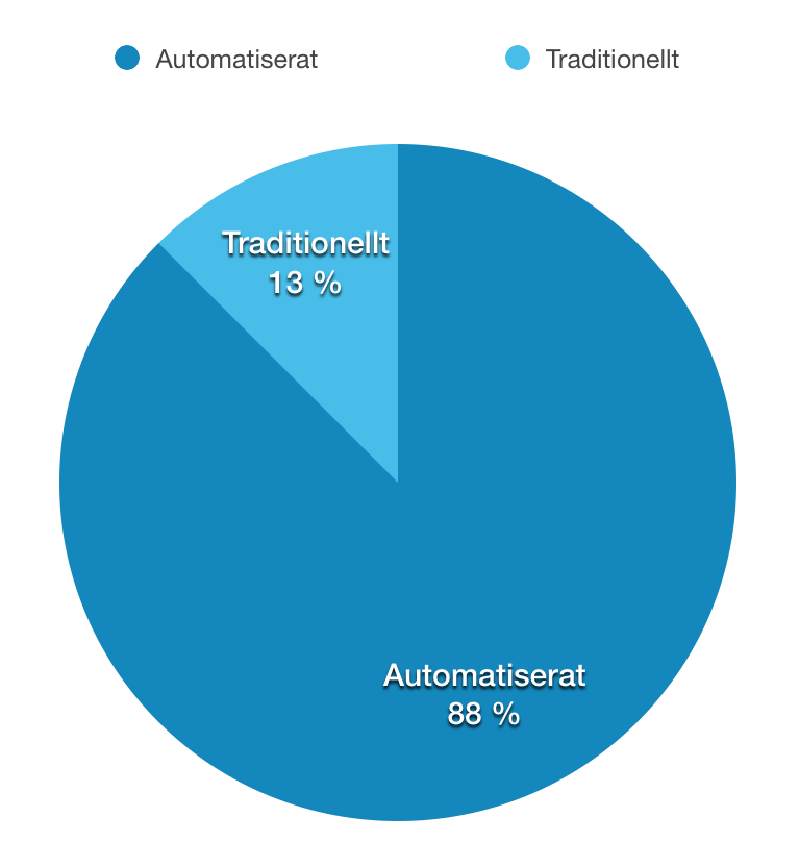
\includegraphics[scale=0.5]{trad_vs_auto.eps}
\caption{Traditionellt eller automatiserat}
\label{fig:TradvsAuto}
\end{figure}

Det är sju av åtta testpersoner som anser att automatiserad bedömning är bättre för deras utveckling som programmerare. Motivering till deras val är fördelarna som nämnts ovanför som snabbare återkoppling och ökad självständighet för studenterna. En testperson menar att ett automatiskt bedömningssystem inte behöver utesluta en labbhandledare eller lärare helt utan mer fungera som ett stöd till dessa. En annan testperson menar att automatiskt och traditionellt bedömningssätt uppfyller olika syften. Testpersonen menar att ett traditionellt bedömningssätt är bättre vid introduktionskurser eftersom det kan krävas mer hjälp och bättre återkoppling. Vidare menar testpersonen att ett automatiserat system är mer lämpligt att använda i kurser med avancerat innehåll eftersom fokus i dessa kurser är problemlösning av specifika problem istället för utlärning inom ett specifikt ämne vilket är fokus i introduktionskurser.

\subsection{Testfallsexperiment}

Här presenteras resultaten från vårt experiment där vi uppmätte tidsåtgången för skapandet av testfall för laborationsuppgifter. Vi valde två stycken laborationsuppgifter från kursen objektorienterad programmering vilka var laboration 13\footnote{Appendix D} och laboration 19\footnote{Appendix E}. För att testfallen som vi skapade ska vara verifierbara krävdes det även att vi implementerade en korrekt lösning för respektive laborationsuppgift. Båda laborationsuppgifterna innehåller deluppgifter vilka representeras med en bokstav, exempelvis laboration 13A. Vi valde att skapa testfall för deluppgifterna A-E för laboration 13 och A-E för laboration 19.  I tabell \ref{tab:Testcase} presenteras tidsåtgången för laborationsuppgifterna, alla tidsåtgångar är angivna i minuter och sekunder. Vi har slagit ihop laborationsuppgift 13B med 13C och 13D med 13E vilket gett namnet 13BC respektive 13DE och de betraktas som deluppgifter.

\begin{table}[h!]
	\centering
	\caption{Resultat från skapandet av kod och testfall}
	\label{tab:Testcase}
	\begin{tabular}{c c c c}
		\toprule
		Laborations nummer & Tid kod & Tid testfall & Total tid\\
		\midrule
		13A & 02,32 & 11,13 & 13,45\\
		13BC & 02,47 & 09,50 & 12,37\\
		13DE & 02,24 & 12,03 & 14,27\\
		\midrule
		19A 	& 03,05 & 05,45 & 08,50\\
		19B & 06,03 & 09,24 & 15,27\\
		19C & 04,44 & 10,13 & 14,57\\
		19D & 01,02 & 03,17 & 04,19\\
		19E & 02,51 & 06,35 & 09,26\\		
		\bottomrule
	\end{tabular}
\end{table}
Tidsåtgången för att skapa testfall varierar beroende på hur uppgiften är definierad och strukturerad men ingen deluppgift överstiger 12 minuter. Den högsta totala tiden för en deluppgift är 15 minuter och 27 sekunder och den lägsta är 4 minuter och 19 sekunder samt medelvärdet för en deluppgift är 11 minuter och 43 sekunder. Den totala tiden, vilket innefattar skapandet av kod och testfall, för laboration 13 är 40 minuter och 49 sekunder respektive 52 minuter och 59 sekunder för laboration 19 vilket tillsammans är 93 minuter och 48 sekunder. Medelvärdet för en laboration är 46 minuter och 54 sekunder.

\newpage
\section{Analys och diskussion}

\textbf{Nedanför presenteras våra tankar kring vad vår analys och diskussion kan komma att innehålla. Observera att det endast är tankar och mer noggranna uträkningar kommer givetvis att genomföras senare. Se det som en förhandsvisning för hur denna del kan komma att se ut. Observera även att vi kommer att ha mer analys och diskussion än det som vi nämner nedanför.}
\\
\\
Lärarna tror inte riktigt på att använda ett bedömningssystem i programmeringskurser på grund av att de tror att det är svårt att bedöma om studenten har uppnått tillräcklig förståelse. Två av lärarna ser inte möjligheten att använda ett bedömningssystem.

Lärarna lyfte under intervjuerna fram en önskan om att kunna använda quiz som ett verktyg för att testa studenternas kunskaper och utmana dem till att lära sig teorin på egen hand. Detta fick oss att börja tänka på hur vi kan använda oss av detta i vår prototyp och vi tog fram en lösning där läraren har möjlighet att vid skapandet av en uppgift i prototypen lägga till ett quiz som studenten måste avklara innan personen har möjlighet att ladda upp sin programmeringslösning. Vi funderade även kring om när det var bäst att använda ett quiz, innan uppladdning av programmeringslösning, efteråt eller både och. Resultaten från enkäten som testpersonerna fick besvara visade att ungefär hälften tyckte att det räckte med att ha ett quiz före uppgiften för att avgöra om studenten uppnått tillräcklig förståelse. Den andra hälften tyckte att man bör använda ett quiz både före och efter uppgiften. De nämnde att genom att använda ett quiz efteråt så kan man exempelvis ställa djupare frågor om teorin för att verkligen säkerställa att studenten uppnått tillräcklig förståelse. Då ett quiz ger denna möjligheten kan lärarnas anledning till varför dem inte tror på att använda ett bedömningssystem lösas eftersom det då är möjligt att kontrollera att studenten uppnått tillräcklig förståelse.
\\
\\
Genom våra experiment där vi skrev testfall och uppmätte tidsåtgången visar det tydligt att genom att använda ett bedömningssystem kan det minska lärares resursanvändning för bedömning otroligt mycket.

Genom att vi från intervjuerna tog reda på att i en kurs läggs 180 minuter per student på att rätta programmeringsuppgifter, kursen det gäller är objektorienterad programmering som är på 15 hp. 

Vi har inte fått exakt data på hur många studenter som registreras för kursen objektorienterad programmering och hur många studenter som klarar kursen, detta är dock något som vi ska ta reda på, vilket borde vara enkelt genom att kontakta studieadministratören.

Men om vi antar att det är ungefär 120 studenter i kursen, ger detta 21600 minuter som läggs på att rätta programmeringsuppgifter, uträkningen är 180 minuter * 120 studenter. 21600 minuter ger 360 timmar vilket är 15 dygn.

Detta kan jämföras mot vår resultat av testfallen där medelvärdet för en laboration är 46 minuter och 54 sekunder, vilket vi kan avrunda till 47 minuter för enklare uträkning.

I kursen objektorienterad programmering är det 16 stycken laborationer, vilket ger en total tid på 752 minuter för samtliga laborationer, vilket motsvarar 12 timmar och 32 minuter.

Medelvärdet som läggs på att rätta en programmeringsuppgift är 180 minuter / 16 laborationer vilket ger 11 minuter och 15 sekunder, vilket kan avrundas till 11 minuter. Om vi fortfarande antar att det är 120 studenter ger det 1320 minuter som läggs på att rätta en laborationsuppgift för samtliga studenter, vilket i timmar är 22 och det är enbart för en laboration, detta kan jämföras med den tid som vi uppmätte där en laboration i medelvärdet tar 46 minuter och 54 sekunder att skapa, om vi säger att det tar en timme att skapa en laboration med testfall, är det 22 gånger så mycket mer tid som läggs på att rätta en laboration.

Detta visar att ett bedömningssystem kommer minska tiden för en lärare när det kommer till bedömningen. Men vi kommer även att diskutera kring om detta är bästa sättet ur studenternas perspektiv.
\\
\\
Angående vårt system hade vi som tanke att använda Git eller något annat versionshanteringssystem för inlämning av uppgifter och en eventuell push skulle trigga systemet att rätta uppgiften. Vi valde inte att använda oss av detta för att lärarna ansåg att det är ett hinder i deras utveckling och för att vi har hittat teori som även stödjer detta. Denna teori tänker vi lyfta fram här i analys och diskussionsdelen.

Vi kommer även att diskutera kring de olika tekniker som vi använder i vår prototyp, speciellt docker eftersom det är genom detta som vi kan exekvera studentens program i en virtuell säker miljö.

Vi kommer även analysera om testfall är ett bra sätt att bedöma students program, eller om det finns andra sätt som är bättre att använda.
\\
\\
De testpersoner som genomförde experimentet ställde sig väldigt positiva till att använda ett bedömningssystem vid programmeringskurser för att de får direkt återkoppling, vilket vi även har teori, som vi ska ta med här i analys och diskussionsdelen, som påvisar att direkt återkoppling gör att personer lär sig mer och snabbare.

Det negativa som testpersonerna lyfte fram med vår prototyp var att återkopplingen var svår att förstå, de upplevde dock att detaljnivån var bra men att vi borde strukturera och presentera det på ett bättre sätt. Med mer implementationstid tror vi att detta problem går att lösa.

Vi fick många intressanta aspekter och åsikter från de testpersoner som medverkade i experimenten som vi kommer att lyfta fram och diskutera kring och vi kommer att använda oss av teori som vi har för att stödja påstående och vår analys.

En intressant åsikt som en testperson lyfte fram var att bara för att det finns en labbhandledare behöver det inte betyda att deras återkoppling är bättre än ett bedömningssystem, det krävs att labbhandledare har bra kunskaper om det som ska läras ut om det ska hjälpa studenten.

\newpage
\section{Slutsatser och vidare forskning}


%
% Do not change
\newpage
\addcontentsline{toc}{section}{Referenser}

\bibliographystyle{ieeetr}
\bibliography{referenser}

\newpage

% Före Enkät
\includepdf[pages=1,scale=0.7,pagecommand=\section*{Appendix A}]{enkat_fore.pdf}
\includepdf[pages=2-,scale=0.7,pagecommand={}]{enkat_fore.pdf}

% Efter Enkät
\includepdf[pages=1,scale=0.7,pagecommand=\section*{Appendix B}]{enkat_efter.pdf}
\includepdf[pages=2-,scale=0.7,pagecommand={}]{enkat_efter.pdf}

% Intervjufrågor
\includepdf[pages=1,scale=0.7,pagecommand=\section*{Appendix C}]{intervjufragor.pdf}

% Labb 13
\includepdf[pages=1,scale=0.7,pagecommand=\section*{Appendix D}]{labb_13.pdf}
\includepdf[pages=2-4,scale=0.7,pagecommand={}]{labb_13.pdf}

% Labb 19
\includepdf[pages=1,scale=0.7,pagecommand=\section*{Appendix E}]{labb_19.pdf}
\includepdf[pages=2-5,scale=0.7,pagecommand={}]{labb_19.pdf}

\end{document}